% Template for FMI-2011 paper; to be used with:
%          fmiconf.sty - LaTeX style file, and
%          IEEEbib.bst - IEEE bibliography style file.
% --------------------------------------------------------------------------
\documentclass{article}
\usepackage{fmiconf,amsmath,epsfig}

\usepackage{german}
\usepackage[utf8]{inputenc}
\usepackage{url}

% Example definitions.
\def\x{{\mathbf x}}
\def\L{{\cal L}}

% Title.
\title{Kann eine Flugdrohne präzise nur mit den Sensoren eines Smartphones gesteuert werden?}
\name{Stefan Baumann, Florian Gümbel}
\address{Technische Hochschule Mittelhessen}

\begin{document}
\maketitle
\begin{abstract}
\glqq Drohne\grqq{} ist mittlerweile auch im Konsumbereich ein fest etablierter Begriff, der ein mit motorisierten Propellern angetriebenes Flugobjekt beschreibt. Die Steuerung erfolgt zumeist über eine Anwendung auf Smartphone / Tablet. Dabei wird hauptsächlich ein virtuelles Joypad auf dem Bildschirm angezeigt das mit Gesten gesteuert wird.\\ Eine andere aber bisher weitestgehend eingeschränkt genutzte Art der Steuerung ist der Einsatz von Lage- und Beschleunigungssensor des Smartphones. Eingeschränkt insofern, da nicht alle Möglichkeiten der Sensoren genutzt werden. An diesem Ansatz soll mit der Entwicklung einer nativen Android Anwendung für Smartphones angeknüpft werden. Ziel ist es, die Bewegungen, die vom Benutzer mit dem Smartphone getätigt werden, an die Drohne zu übertragen. Am Ende gilt es die Frage zu beantworten, ob die Steuerung einer Drohne präzise genug ist, wenn diese komplett über Lage- und Beschleunigungssensor des Smartphones erfolgt.

\end{abstract}

\section{Einleitung}
\label{sec:einleitung}
Im Konsumbereich nimmt die Beliebtheit von sogenannten Drohnen immer mehr zu. Diese neue Form des unbemannten Flugobjektes zeichnet sich zumeist dadurch aus, dass sie, anders als herkömmliche bekannte Modellflugzeuge, mindestens vier kleine Propeller hat, welche über Elektromotoren angetrieben werden und die Drohne senkrecht starten lassen. Die Anzahl der Propeller kann variieren. Angefangen von Quadrocopter über Hexacopter und Octacopter bis hin zu Multicopter. Der Einsatzzweck einer solchen Drohne geht von Vermessungstechnik über Luftaufnahmen und Erkundung bis hin zur Jagd. In folgenden geht es jedoch um die für die im Privatverbrauch übliche Hobby-Flugdrohne.

Um eine Solche Drohne zu steuern gibt es verschiedene Möglichkeiten. Abhängig von Modell lassen sich klassische Fernsteuerungen\cite{flypad} entweder direkt mit der Drohne Verbinden oder über Umweg mit Hilfe einer App.Jeder Drohnenhersteller bietet auch eine eigene App für alle gängigen Smartphones oder Tablets an. Die Verbindung findet je nach Modell über W-Lan oder Bluetooth statt. Für die Steuerung mittels App auf dem Gerät stehen in der bekanntesten Variante meist zwei digitale Joysticks zur Verfügung deren Bewegung umgerechnet und auf die Drohne übertragen wird während das Gerät ruhig in der Hand liegt. Meistens ist über den linken Joystick die Veränderung der Höhe und eine Drehung möglich. Der rechte Joystick ist für die horizontale Bewegung zuständig. Damit ist das Schwenken zur Seite sowie das vorwärts- und rückwärts fliegen gemeint. Eine schwerere Variante der Steuerung ist die Richtungsangabe mittels Neigung des Gerätes.

Die Idee ist es nun, eine Erweiterung der schweren Variante zu untersuchen, bei der zwei Sensoren des Smartphones zum Einsatz kommen. Dabei soll komplett auf die Bedienung von Touchscreen verzichtet und nur das Gerät selbst als Steuerungseinheit verwendet werden. Dazu dienen die beiden Sensoren (Lage- und Beschleunigungssensor) zur Erfassung der Bewegungen\cite{milker2012bewegungserkennung} woraufhin das Smartphone diese umrechnet und auf die Drohne überträgt. 

\section{Stand der Technik}
\label{sec:verwandteArbeiten}
\subsection{Drohnensteuerung}
Neben einigen sehr wenigen Drittherstelleranwendungen bieten, wie bereits in der Einleitung erwähnt, auch die Hersteller der Drohnen eigene Anwendungen zum steuern der Drohne an.

Die bekannte Firma Parrot stellt eine Vielzahl verschiedener Apps zum steuern bereit. Eine davon ist die FreeFlight-App \cite{freeflightapp}, die eine Steuerung durch den Gyroscope-Sensor unterstützt. Insgesamt bietet sie drei Möglichkeiten an, wobei der linke Joystick immer für die Höhe und Drehung zuständig ist:
\begin{description}
\item Normal \\
Wie in Abbildung \ref{fig:freeflight} dargestellt, wird auf dem rechten Joystick ein Symbol angezeigt, auf das dauerhaft gedrückt werden muss um die Flugrichtung der Drohne mit Neigung des Smartphones anzugeben.
\item Ass (Experte) \\
Auf dem rechten Joystick kann eine schnelle Kursänderung mittels Swipe-Geste angegeben werden, während durch drücken des linken Joysticks und neigen des Smartphone eine Änderung der Flugrichtung erzielt werden kann.
\item Joypad\\
Hierbei handelt es sich um die standardmäßige Steuerung der Drohne mittels der beiden Joysticks.
\end{description}

Bei Normal und Ass fliegt die Drohne in die Richtung in der das Smartphone geneigt wird ohne sich dabei in diese zu drehen. Eine Höhenveränderung oder Drehung durch Bewegung ist in keiner Variante möglich. 

\begin{figure}[htb]
\begin{minipage}[b]{1.0\linewidth}
  \centering
\centerline{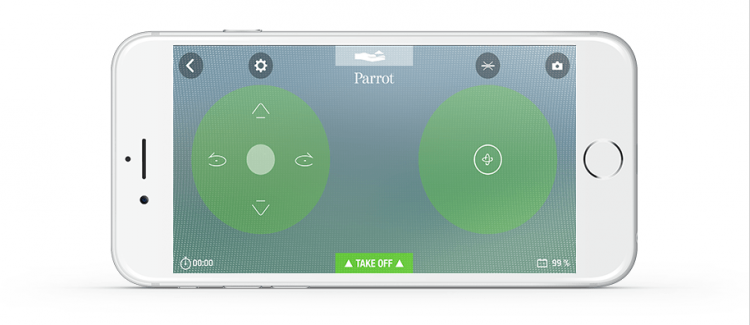
\includegraphics[width= 85mm]{freeflight_mini.png}}
\end{minipage}
\caption{Normale Steuerung (Quelle: Parrot)}
\label{fig:freeflight}
\end{figure}

Bereits Anfang 2015 hat Sony ein Projekt vorgestellt, in dem eine Drohne mittels SmartWatch 2, SmartEyeglass und Smartphone gesteuert wird \cite{sonyflight}. In diesem Fall ist die Smartwatch via Bluetooth mit dem Smartphone verbunden und überträgt die Bewegung per W-Lan an die Drohne. Über das Display der Smartwatch lassen sich dabei die verschiedenen Steuerungs-Modi umschalten. Hier kommen sowohl Accelerometer als auch Gyroscope zum Einsatz.

\subsection{Einsatz von Sensoren}
Die in Abbildung \ref{fig:gyro} gezeigten Sensoren finden in vielen Bereichen Verwendung und sind bereits in jedem aktuellen Smartphone standardmäßig verbaut. 
Sie werden meistens in Kombination genutzt wie beispielsweise bei der Erkennung von Bewegungsänderung oder der Messung von physikalischen Aktivitäten \cite{wu2012classification}. Auch bei Spielen sind sie ein gern genutztes Hilfsmittel. Etwa um in Rennspielen das Lenken eines Fahrzeuges zu simulieren oder einen Balanceakt zu meistern.
Um die derzeitige Beschleunigung des Gerätes zu ermitteln, kommt das Accelerometer oder auch Beschleunigungssensor zum Einsatz. Mittels der Schwerkraft wird ermittelt, in welche Richtung das Smartphone bewegt wird. In der Regel kommen die X- Y- und Z-Achse zum Einsatz. Die Lage und somit auch die Drehbewegung des Smartphones wird vom Gyroscope oder Magnetometer gemessen. Beim Gyroscope wird die Corioliskraft und das sogenannte Stimmgabelprinzip genutzt. Das Magnetometer greift auf die Stärke des Erdmagnetfelds zurück. Hier kommen Längs-, Quer- und Hochachse für die Positionsbestimmung im Raum zum Einsatz.
\begin{figure}
\begin{minipage}[b]{1.0\linewidth}
  \centering
\centerline{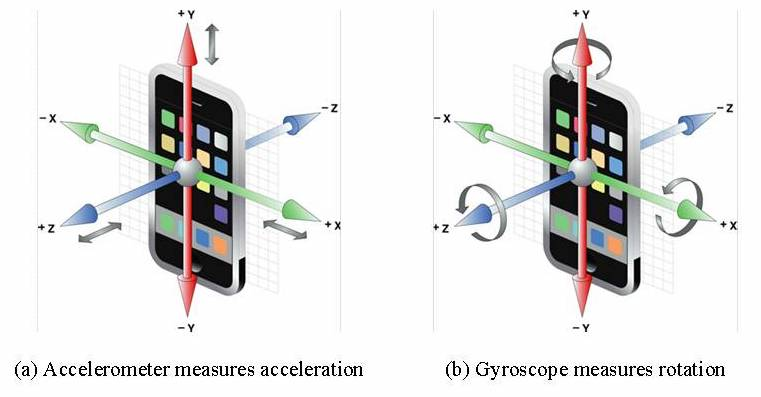
\includegraphics[width= 85mm]{gyro.jpg}}
\end{minipage}
\caption{Accelerometer und Gyroscope (Quelle: Apple Inc.)}
\label{fig:gyro}
\end{figure}

\section{Methodik}

\subsection{Eingesetzte Drohne}
Als Testdrohne kam eine Parrot Airborne Night Drone der Kategorie Mini-Drohne zum Einsatz\cite{minidrone}, da sie folgende Vorteile mit sich bringt:
\begin{itemize}
	\item Relativ geringen Anschaffungspreis
	\item Unterstützung des aktuellen Parrot SDK3
	\item Gute Testbarkeit in Gebäuden durch geringe Größe 
\end{itemize}

Weiterhin verfügt die Drohne über zwei LED- Suchscheinwerfer, einen 1GB Flashspeicher für Fotos mit der eingebauten VGA(640x480) Mini-Kamera, einen Ultraschall-Reichweitenmesser sowie ein 3-Achsen-Gyroscope und einen 3-Achsen-Beschleunigungsmesser (+\/- 50mg).

Nach einer Flugzeit von maximal 9 Minuten (ohne Schutz) kann der 550 mAh-Akku mittels Quickcharging in 25 Minuten aufgeladen werden.

\subsection{Verwendete Technologien}
Wie in den vorangegangenen Kapiteln schon erläutert wurde, gibt es aktuell keine App die eine komplette Steuerung über die Sensoren unterstützt. Aus diesen Gründen wurde zu Testzwecken ein Prototyp entwickelt, welcher die gestellten Anforderungen erfüllt. Aus Gründen der Flexibilität wurde sich, für die Umsetzung des Prototypen, für eine native Android-Anwendung zusammen mit dem SDK3 von Parrot entschieden.

Als Verbindung kommt bedingt durch die Drohne Bluetooth in der Version 4.0 zum Einsatz. Während größere Drohnen W-Lan anbieten, beschränkt sich die Minidrohnen-Reihe auf Bluetooth. Dadurch ist die Reichweite der Drohne auf 20 Meter begrenzt, was angesichts der kleinen Größe und der Nutzung in Gebäuden keinen Nachteil darstellt.

\subsection{Zielgruppenbestimmung}
Eine Einschränkung der Zielgruppe ergibt sich aus der Entwicklung des Prototyps für die Parrot Airborne Night-Reihe oder andere Parrot Flugdrohnen die mittels Bluetooth verbunden werden. Zusätzlich ist die Nutzung auf Android-fähige Smartphones in der Version 6.0.1 oder höher beschränkt. Ansonsten kann jeder, der diese Einschränkungen erfüllt, und Interesse an einer alternativen Steuerungsmethode hat zur Zielgruppe gezählt werden.
  
\subsection{Vorgesehene Steuerung}
Die sinnvolle Erweiterung der bereits bestehenden Steuerung ist die Kernaufgabe des Prototyps. Mit einer guten Umsetzung kann ein präzises steuern nur mit Sensoren möglich sein. Wie bereits in Kapitel 3.2 beschrieben, haben beide Sensoren verschiedene Eigenschaften die sie liefern. Diese gilt es nun so einzusetzen, dass eine Steuerung durch Bewegungen so einfach wie möglich ist. Grundsätzlich gibt es an der bisher von Parrot zur Verfügung gestellten Form der Steuerung durch Bewegung nichts zu kritisieren. Sie ist vom Prinzip her logisch aufgebaut, sodass der Benutzer sie intuitiv bedienen kann ohne vorher eine Betriebsanleitung lesen zu müssen.

Daraus ergibt sich, dass zwei der drei Achsen des Lagesensors schon in Verwendung sind. Nimmt man die Verteilung der in Abbildung \ref{fig:gyro} gezeigten Sensoren an, so ist die X-Achse bereits für die Seitliche Bewegung und die Y-Achse für Vor und Zurück der Drohne zuständig. Als erste Neuerung soll die Z-Achse genutzt werden um die Funktion zum Drehen des linken Joysticks zu implementieren. 

Eine weitere Funktion des linken Joysticks ist die Änderung der Höhe. Hierfür eignet sich besonders die in Abbildung \ref{fig:gyro} gezeigte Z-Achse des Accelerometer. Ebenfalls kann durch eine schnelle Auf-Bewegung die Drohne starten und durch eine schnelle Abwärts-Bewegung landen. Aber auch die Swipe-Funktionen aus der Experten Variante sollen mittels Accelerometer umgesetzte werden. Die 90 Grad-Drehung kann durch eine rasche Bewegung in die jeweilige Richtung ausgelöst werden. Eine schnelle Bewegung nach vorne sorgt für eine 180 Grad-Drehung über die linke Seite und eine schnelle Bewegung nach hinten für eine über die rechte Seite. Abbildung \ref{fig:gameplay} zeigt grafisch wie die Steuerung mit Sensoren aussehen soll. 

\begin{figure}
\begin{minipage}[b]{1.0\linewidth}
  \centering
\centerline{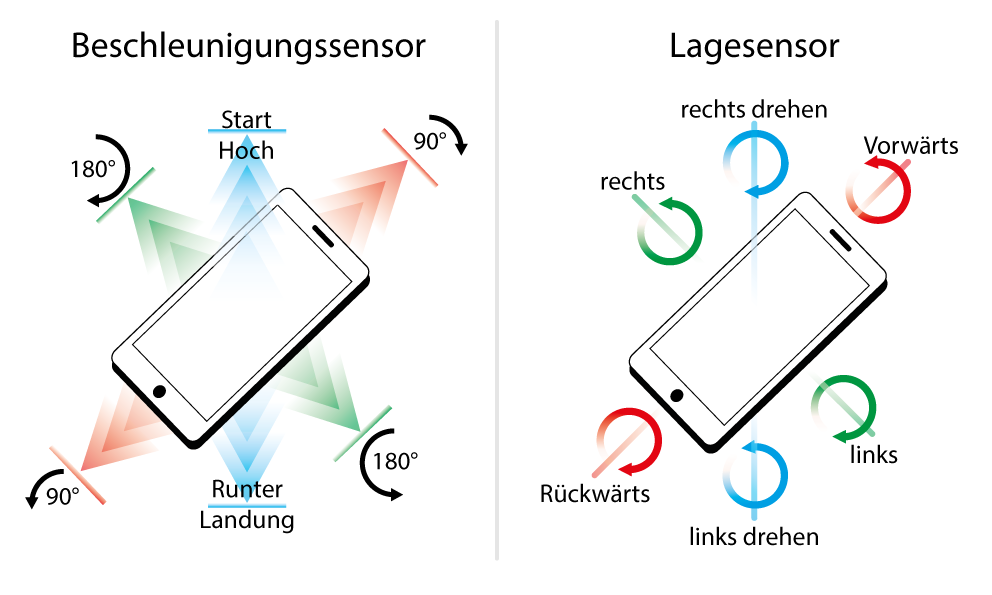
\includegraphics[width= 85mm]{gameplay}}
\end{minipage}
\caption{Steuerung mit Sensoren}
\label{fig:gameplay}
\end{figure}


Streng genommen könnte auch das Auslösen der Kamera oder das Einschalten der LED zur Steuerung gehören. Da es sich bei den Tests aber um das reine Fliegen handelt werden diese bei dem Prototyp nicht berücksichtigt.

\subsection{Umsetzung des Prototypen}
Als Platform des Prototypen wurde Android gewählt. Das von Parrot zur Verfügung gestellte SDK verlangt als Mindestanforderung die Android API 23, welches Android 6 entspricht.
Somit grenzt sich der Einsatzbereich der App auf neue Android-Versionen ein.\\
Als Grundlage für die Android-App kommt die Beispiel-Anwendung von Parrot zum Einsatz. Diese bot den Vorteil, dass die Implementierung des Verbindungsaufbaus bereits vorhanden war.

Wie bereits erläutert, wird die Steuerung mit Hilfe des Geomagnetfeld-Sensors sowie dem Accelerometer umgesetzt. Für beide Sensoren wurden jeweils eine Controller-Klasse implementiert,
die speziell den Steuerungsanteil des Sensors für die Drohne übernimmt.
Der Geomagnetfeld-Sensor ist verantwortlich für die Steuerung der Drohne durch Kippen und Neigen des Smartphones und somit für die Bewegungsrichtung der Drohne.
Vorteil der Verwendung des Geomagnetfeld-Sensors ist die leichtere Verarbeitung der daraus resultierenden Daten.\\
Das Accelerometer wird verwendet, um Beschleunigungs-Bewegungen (Start, Landung, Swipe) festzustellen.
Zunächst betrachten wir die Auswertung der Geomagnetfeld-Daten: Hierbei liefert der Sensor in zuvor eingestellten Abständen die X-,Y- und Z-Lagen zurück. Es handelt es sich Float-Werte zwischen 1 und -1. Dabei entspricht die jeweilige Grenze einer Drehung von 90 Grad oder -90 Grad um die bestimmte Achse. Diese Werte werden von der Anwendung in Teilabschnitten als Steuerbefehle an die
Drohne weitergereicht. Die Drohne nimmt dabei Werte von -100 bis 100 entgegen, was prozentual der maximalen Neigung entspricht. Für die Einteilung der Werte des Sensors wurden Schritte zwischen
(-)0.15, (-)0.25, \textgreater{} (-)0.25 verwendet. Neigungen mit Werten zwischen (-)0.15 und (-)0.25 wirken eine 40\%ige Neigung, Werte größer (-)0.25 eine 60\%ige Neigung. Für Werte kleiner
(-)0.15 werden als Null-Position angenommen und die Drohnen-Neigung wird auf 0 zurückgesetzt.

Bei der Verarbeitung der Daten des Beschleunigungssensor werden die Werte in eine lineare Komponente und eine Gravitationskomponente aufgeteilt. Die lineare ist stets positiv und ermöglicht eine schnelle Filterung bzw. ein schnelles Stepping zur Steuerung. Die Graviationskomponente dagegen dient als Richtungs-Indikator.
Als Mindest-Grenzwert der linearen Komponente ist 6 festgelegt. Sind lineare Werte größer, erfolgt ein Steuerbefehl an die Drohne in die mit der Beschleunigungsachse verknüpften Richtung.
Dies sind Start und Landung auf der Z-Achse sowie Drehungen von 90 Grad bzw. 180 Grad um die Drehachse der Drohne.

\section{Ergebnisse und Evaluation}
Um die eingangs gestellte Frage ehrlich beantworten zu können, muss eine Evaluation durchgeführt werden in der eine möglichst breite Masse an verschiedenen Personen den Prototyp unter gleichen Bedingungen testet. Hierfür wurde ein Parkour aufgebaut welcher einmal mit den von Parrot gelieferten Steuerungsmöglichkeiten und einmal mit dem entwickelten Prototyp getestet werden muss. Der Parkour ist so aufgebaut, dass alle Funktionen mindestens einmal dran kommen. Die Altersspanne der sieben Probanden lag im Bereich von 11 bis 65 Jahren. Es wurden bewusst Tester ausgesucht, die keinerlei Vorkenntnisse mit dem Fliegen einer Drohne haben.

Zur Einführung wurden die jeweiligen Steuerungsmethoden erklärt. Aus Gründen der Fairness wurde auf vorherige Testflüge verzichtet. Als Ausgangslage wird die Drohne in einem geringen Abstand vor die Testperson auf eine gekennzeichnete Fläche gestellt. In 1 Meter Abständen wurden vier Hütchen aufgestellt. Es galt die Drohne zu starten, sie durch den Slalom zu manövrieren und sie nach einer 180 Grad-Drehung auf eine weitere gekennzeichnete Fläche sicher zu landen.

Anschließend erfolgte die Aufnahme von Meinungen der Testpersonen zusammen mit den Beobachtungen. Diese wurden gebeten, ihr persönliches Empfinden zu schildern, mit welcher Steuerung sie besser zurecht kamen und mit welcher sie ihrer Ansicht nach, präziser können.

Bei der Auswertung stellte sich heraus, dass die Steuerung nur mit Sensoren durchaus Potential hat, ein neuer Steuerungsmodus zu werden. Allerdings erwies sich die prototypische Anwendung in einigen Fällen noch als zu unpräzise, sodass sich die Steuerung mit Hilfe des Joysticks als besser erwies. Jedoch wurden auch die Steuerungsmodi Normal und Ass als gewöhnungsbedürftig und schwieriger empfunden, was auf die Steuerung mit Sensoren zurück zu führen ist. 

\section{Zusammenfassung und Ausblick}
Um herauszufinden, ob es möglich ist eine Drohne präzise nur mit Sensoren des Smartphones zu steuern wurde ein Prototyp entwickelt. Anschließend wurden die verschiedenen Steuerungsmöglichkeiten Personen gegeben und diese nach ihrer Meinung gefragt. Dabei stellte sich heraus, dass die Sensoren-Steuerung besser funktioniert als gedacht aber im Vergleich zu den bereits vorhandenen Möglichkeiten teilweise zu unpräzise ist. 

Daraus ergibt sich, dass die eingangs aufgestellte Fragestellung nicht bestätigt werden kann. Dennoch ist es eine interessante Alternative zu den traditionellen Steuerungsmethoden und kann mit Einbußen der Präzision ohne weiteres genutzt werden.

Eine Fertigung des Prototypen ist nicht geplant.

\bibliography{Template}{}
\bibliographystyle{IEEEbib}
\end{document}